\documentclass[12pt]{report}
\usepackage{pdfpages}
\usepackage{lscape}
\usepackage{hyperref}
\hypersetup{
    colorlinks=true,
    linkcolor=black,
    %filecolor=magenta,      
    urlcolor=black,
    breaklinks=true,
   % citecolor=blue,
}
\usepackage[nottoc,notlof,notlot]{tocbibind} 
\usepackage{framed}
\usepackage{rotfloat}
\usepackage{subfig}
\usepackage{graphicx}
\usepackage{caption} 
%\captionsetup[table]{skip=10pt}
\usepackage{graphicx}
\usepackage[utf8]{inputenc}
\usepackage{verbatim}
\usepackage[utf8]{inputenc}
\usepackage{amsmath}
\usepackage[english]{babel}
\usepackage{float}
\usepackage{tikz}
\usepackage{pgfplots}
\usepackage{pbox}
\usepackage{url}
\usepackage{tkz-graph}
\usetikzlibrary{arrows}
\usepackage{array}
\usepackage{amssymb}
\usepackage{fancyvrb}
\usepackage{listings}
\usepackage{ragged2e}
\usepackage{slashbox}
\makeatletter
\def\BState{\State\hskip-\ALG@thistlm}
\makeatother
\usepackage{sectsty}
\usepackage{comment}
\usepackage{soul}
\usepackage{enumitem}
\usepackage{array}
\usepackage{chngcntr}
\usepackage{cancel}
\usepackage{multirow}
%\usepackage{subfigure}
\usepackage[toc,page]{appendix}
\usepackage{tikz}
\usepackage{setspace}
\usepackage{afterpage}
\usetikzlibrary{shapes,arrows}
\graphicspath{ {images/} }
%\topmargin -23 mm
\providecommand{\keywords}[1]{\textbf{\textit{Keywords---}} #1}
%\headheight 8pt
%\oddsidemargin 0mm
%\evensidemargin -5mm
\textwidth 161mm
\textheight 210mm
\linespread{1}
%\footskip = 60pt
\usepackage{titlesec}
\chapterfont{\centering}
\newcolumntype{P}[1]{>{\centering\arraybackslash}p{#1}}
\newcolumntype{M}[1]{>{\centering\arraybackslash}m{#1}}
\renewcommand{\baselinestretch}{1.3} 
\titleformat{\chapter}[display]   
{\normalfont\huge\bfseries\centering}{\chaptertitlename\ \thechapter}{10pt}{\Huge\centering}   
\titlespacing*{\chapter}{0pt}{-50pt}{5pt}
\usepackage{pdfpages}
\usepackage[linesnumbered,ruled]{algorithm2e}
% ---------------------------------------------------------------------------
% ADDED (compile fix): packages, colours, column types and macros that the
% chapters use but which were never defined. Nothing here changes fonts,
% margins, spacing or any existing style setting.
% ---------------------------------------------------------------------------
\usepackage{longtable}
\usepackage{booktabs}
\usepackage{tabularx}
\usepackage[table]{xcolor}   % provides xcolor + colortbl (\rowcolor, \cellcolor)
\definecolor{softblue}{RGB}{221,235,247}
\definecolor{rowgray}{RGB}{235,235,235}
% colours used by the TikZ diagrams in Chapter 3 (traffic-light style palette)
\definecolor{navy}{RGB}{31,56,100}
\definecolor{softgreen}{RGB}{226,239,218}
\definecolor{softamber}{RGB}{255,242,204}
\definecolor{softred}{RGB}{248,215,218}
\definecolor{softpurple}{RGB}{228,223,236}
\usetikzlibrary{arrows.meta}   % provides the 'Stealth' arrow tip used in Chapter 3
\newcolumntype{L}[1]{>{\raggedright\arraybackslash}p{#1}}   % left, fixed width
\newcolumntype{C}[1]{>{\centering\arraybackslash}p{#1}}     % centred, fixed width
\newcolumntype{Y}{>{\raggedright\arraybackslash}X}          % stretchy left column (tabularx)
\providecommand{\trafma}{TRAF-MA}
\providecommand{\tentative}{$^{\dagger}$}                    % marks a working / tentative choice
% Harvey-ball rating symbols used in the survey comparison table
\newcommand{\hbnone}{\tikz[baseline=-0.6ex]{\draw[line width=0.4pt] (0,0) circle (0.9ex);}}
\newcommand{\hbhalf}{\tikz[baseline=-0.6ex]{\draw[line width=0.4pt] (0,0) circle (0.9ex); \fill (0,0) -- (0,0.9ex) arc (90:-90:0.9ex) -- cycle;}}
\newcommand{\hbfull}{\tikz[baseline=-0.6ex]{\filldraw[line width=0.4pt] (0,0) circle (0.9ex);}}
% ---------------------------------------------------------------------------
\usepackage[  
 top    = 1.5in,
  bottom = 1in,
  left   = 1.5in,
  right  = 1in, 
  %headsep=5mm,%%% Example
  %includeheadfoot%%%%%%%%%%%%%%%%%%%%%%%%%%
  ]{geometry}
%below code used for page bordering
\iffalse
\usepackage{pgf}
\usepackage{pgfpages}0
\pgfpagesdeclarelayout{boxed}
{
  \edef\pgfpageoptionborder{4pt}
}
{
  \pgfpagesphysicalpageoptions
  {%
    logical pages=1,%
  }
  \pgfpageslogicalpageoptions{1}
  {
    border code=\pgfsetlinewidth{1.5pt}\pgfstroke,%
    border shrink=\pgfpageoptionborder,%
    resized width=.95\pgfphysicalwidth,%
    resized height=.95\pgfphysicalheight,%
    center=\pgfpoint{.5\pgfphysicalwidth}{.5\pgfphysicalheight}%
  }%
}
\pgfpagesuselayout{boxed}
\setlength{\parindent}{2cm}
\usetikzlibrary{calc}
\usepackage{eso-pic}
\fi

\begin{document}
% Cover, declaration, certificate and acknowledgement are unnumbered.
\renewcommand*{\thepage}{cover-\arabic{page}}
\pagestyle{empty}
\counterwithin{table}{section}
\counterwithin{figure}{section}
\iffalse
\AddToShipoutPictureBG*{%
\begin{tikzpicture}[overlay,remember picture]
\draw[line width=4pt]
    ($ (current page.north west) + (1cm,-1cm) $)
    rectangle
    ($ (current page.south east) + (-1cm,1cm) $);
\draw[line width=1.5pt]
    ($ (current page.north west) + (1.2cm,-1.2cm) $)
    rectangle
    ($ (current page.south east) + (-1.2cm,1.2cm) $);
\end{tikzpicture}
}
\fi
 \begin{center}
	Major Project-I Report on\\
	\null
	\textbf{\large \textbf{TRAF-MA: A Privacy-Preserving, Trust-Aware Multi-Agent Traffic Intelligence System }}\\
	\null
	
	Submitted in partial fulfillment of the requirements for the degree of\\
	\null
	BACHELOR OF TECHNOLOGY\\
	in\\
	INFORMATION TECHNOLOGY\\
		by \\
	\textbf{Harshul Jain (231IT025)}
	\\\textbf{Laxminarayan Sahu  (231IT035)}
	\\\textbf{{Shubhrodipto De (231IT070)}}\\
	\vspace{0.8em}
	\large{\textit{under the guidance of}} \\
	\vspace{0.8em}
	
	\large{\textbf{Dr. Kiran Manjappa}}\\
	\begin{figure}[h] % b - bottom, t - top, h - here
		\centering{
			
\includegraphics[width=6cm, height=6cm]{symbol.jpg}
		}
	\end{figure}
DEPARTMENT OF INFORMATION TECHNOLOGY\\
NATIONAL INSTITUTE OF TECHNOLOGY KARNATAKA\\
SURATHKAL, MANGALORE - 575025\\
NOVEMBER, 2026\\
\end{center}
\clearpage

\begin{framed}
	\begin{center}
		\textbf{{\Large DECLARATION}}\\
	\end{center}
	\null
	I/We hereby \textit{declare} that the Major Project-1 (IT449) Work Report entitled \textit{\textbf{"TRAF-MA: A Privacy-Preserving, Trust-Aware Multi-Agent Traffic Intelligence System"}},  which is being submitted to the \textbf{National Institute of Technology Karnataka, Surathkal}, for the award of the Degree of Bachelor of Technology in Information Technology, is a \textit{bonafide report of the work carried out by me/us.} The material contained in this Project Report has not been submitted to any University or Institution for the award of any degree.
	\\
	\\
	\textit{Name of the Student (Registration Number) with Signature }
	\begin{enumerate}[label={(\arabic*)}]
		\item  Harshul Jain  (231IT025)
		\item  Laxminarayan Sahu  (231IT035)
		\item  Shubhrodipto De  (231IT070)
	\end{enumerate}
	\null
	Department of Information Technology \\
	Place     : NITK, Surathkal-575025 \\
	Date      :  
	\\
	\\
	\\
	\\
	\\
	\\
	\\
	\\
	\\
	\\
\end{framed}
\clearpage
\begin{framed}
	\begin{center}
		\textbf{{\Large CERTIFICATE}}
	\end{center}
	\null
	This is to \textit{certify} that the Major Project-I (IT449) Work Report entitled \textit{\textbf{"TRAF-MA: A Privacy-Preserving, Trust-Aware Multi-Agent Traffic Intelligence System"}} submitted by \\
	\\
	\textit{Name of the Student (Registration Number)}
	\begin{enumerate}[label={(\arabic*)}]
		\item  Harshul Jain (231IT025)
		\item  Laxminarayan Sahu (231IT035)
		\item  Shubhrodipto De (231IT070)
	\end{enumerate}
	as the record of the work carried out by them, is \textit{accepted as the B.Tech. Project work report submission} in partial fulfillment of the requirement for the award of the degree of \textbf {Bachelor of Technology} in Information Technology.
	\\
    \\
	\begin{minipage}{14cm}
		\begin{center}                                      	\vspace{1.5cm}	
			\textbf{Signature of Major Project Guide with date}
            \\Dr. Kiran Manjappa
            \\Assistant Professor \\
			Department of Information Technology, NITK Surathkal \\
			\end{center}       
     \vspace{0.75cm}
        \begin{center}                                      	\vspace{1.5cm}	
			\textbf{Chairman - DUGC}
            \\{Signature with Date and Seal}
          	\end{center} 
	\end{minipage}
\\
\\
\\

\end{framed}
\thispagestyle{empty}
\clearpage

\clearpage
\begin{center}
	\textbf{{\Large ACKNOWLEDGEMENT}}\\
    \thispagestyle{empty}
\end{center}
\justifying
We wish to express our sincere gratitude to our project guide, \textbf{Dr. Kiran Manjappa}, Department of Information Technology, National Institute of Technology Karnataka, Surathkal, for his valuable guidance, constant encouragement and the freedom he gave us to explore the problem in our own way. His suggestions at every stage, from narrowing the topic to shaping the methodology, have been instrumental in giving this work its present direction.

We are grateful to the Head of the Department and to the faculty members of the Department of Information Technology for their support and for the facilities extended to us during the course of this work. We also thank the members of the Departmental Undergraduate Committee for their review and feedback.

We thank our friends and classmates for the many useful discussions that helped us refine our ideas.

Finally, we thank our families for their patience and encouragement throughout.

\vspace{1.5em}
\begin{flushright}
	\textbf{Harshul Jain (231IT025)}\\
	\textbf{Laxminarayan Sahu (231IT035)}\\
	\textbf{Shubhrodipto De (231IT070)}
\end{flushright}
\clearpage
\clearpage

\hypersetup{pageanchor=false}
\pagenumbering{roman}
\pagestyle{plain}
\chapter*{ABSTRACT}
\addcontentsline{toc}{chapter}{ABSTRACT}
\justifying
Intelligent Transportation Systems increasingly use federated learning (FL) to let vehicles and infrastructure jointly train traffic-prediction models without sharing raw data. However, data locality alone does not guarantee reliability: faulty or malicious agents may submit false traffic reports or poisoned model updates. The problem is especially important in traffic settings because agents genuinely observe different parts of the road. Disagreement between honest agents is therefore expected and must not be mistaken for misbehaviour. Existing FL security and vehicular-trust techniques address parts of this problem, but a coordinated approach is needed to distinguish legitimate disagreement from attacks and to connect trust with both learning and traffic-state consensus.

The overall project addresses this problem through TRAF-MA, a trust-aware multi-agent architecture for a signalised intersection. Its intended design combines heterogeneous vehicle and traffic-signal agents, lightweight local models for congestion classification and queue-length regression, a shared feature representation, and an edge coordinator. The planned trust engine uses contextual, physical and prediction consistency, model-update quality, network reliability and temporal behaviour. Relevance weighting is intended to account for spatial, temporal and coverage differences. Trust is planned to inform both federated aggregation and traffic-state consensus, and to support anomaly handling, quarantine and recovery under false-observation and model-poisoning attacks. The project also aims to evaluate this system in SUMO and integrate it with a real-time monitoring dashboard.

This report is an interim implementation account toward those continuing project objectives. The work completed so far includes the SUMO/TraCI intersection and bounded agents, future queue and congestion labels, compact dataset preparation, a two-head GRU, baseline and central training, and hierarchical FedAvg with an RSU self-update ablation. In the saved 100-vehicle experiment, the central GRU achieved MAE 18.51 m, RMSE 28.28 m, macro-F1 0.764 and balanced accuracy 0.746 on 300 overlapping held-out windows. Hierarchical FL achieved macro-F1 0.342 with RSU learning enabled and 0.298 with it disabled. These are single-seed results from the current simulation; they do not establish the effectiveness of the planned trust, attack, recovery or dashboard components. The report therefore preserves the overall project problem and objectives while presenting methodology and results for the implementation completed to date.

\textbf{Keywords:} Federated Learning, Intelligent Transportation Systems, Trust Management, Multi-Agent Systems, Traffic Prediction, Traffic-State Consensus, SUMO Simulation.

\renewcommand*{\contentsname}{\MakeUppercase{Contents}}
\renewcommand*{\listfigurename}{\MakeUppercase{List of Figures}}
\renewcommand*{\listtablename}{\MakeUppercase{List of Tables}}
\renewcommand{\bibname}{REFERENCES}
\tableofcontents
\clearpage

\begingroup
\addcontentsline{toc}{chapter}{LIST OF FIGURES}
\listoffigures
\clearpage
\endgroup

\begingroup
\addcontentsline{toc}{chapter}{LIST OF TABLES}
\listoftables
\clearpage
\endgroup

\chapter*{LIST OF ABBREVIATIONS}
\addcontentsline{toc}{chapter}{LIST OF ABBREVIATIONS}
\begin{center}
\renewcommand{\arraystretch}{1.35}
\begin{tabular}{@{}p{3.2cm}p{9.5cm}@{}}
\textbf{CE} & Cross-entropy\\
\textbf{FedAvg} & Federated Averaging\\
\textbf{FL} & Federated Learning\\
\textbf{GRU} & Gated Recurrent Unit\\
\textbf{HFL} & Hierarchical Federated Learning\\
\textbf{I2C} & Infrastructure-to-Coordinator (RSU to edge coordinator link)\\
\textbf{IID} & Independent and Identically Distributed\\
\textbf{ITS} & Intelligent Transportation Systems\\
\textbf{JSD} & Jensen--Shannon Divergence\\
\textbf{MAE} & Mean Absolute Error\\
\textbf{RMSE} & Root Mean Squared Error\\
\textbf{RSU} & Roadside Unit\\
\textbf{SUMO} & Simulation of Urban MObility\\
\textbf{TPR / TNR} & True-Positive Rate / True-Negative Rate\\
\textbf{TraCI} & Traffic Control Interface\\
\textbf{TV} & Total Variation (distance)\\
\textbf{V2I} & Vehicle-to-Infrastructure\\
\textbf{VANET} & Vehicular Ad-hoc Network\\
\end{tabular}
\end{center}

\clearpage

\renewcommand{\chaptername}{CHAPTER}
\clearpage
\hypersetup{pageanchor=true}
\pagenumbering{arabic}
\setcounter{page}{1}
% ===================================================Chapter 1===============================================================
\chapter{INTRODUCTION}\label{ch:intro}

\section{Background and Motivation}
Urban intersections bring traffic streams, signal changes, and vehicle interactions together in a small area. Congestion at an intersection is dynamic: queues build during red phases, discharge during green phases, and differ by approach. A useful prediction system therefore needs recent traffic observations and a clear definition of what each observer can see.

Federated learning (FL) is a way to train a shared model while keeping each participant's training examples at that participant. Clients send model updates to an aggregator rather than uploading raw histories. This addresses a data-sharing concern, but it is not a formal privacy guarantee: model updates can still reveal information, and an aggregator cannot infer whether an update is reliable from its weights alone. Federated averaging (FedAvg) provides a simple and inspectable starting point for collaborative model training \cite{mcmahan2017}.

Traffic data also vary by place and observer. A roadside unit (RSU) measures an approach zone; a vehicle observes its own state and nearby vehicles on the road it is travelling. Even honest clients may therefore have different feature availability and label distributions. Such differences are a non-independent and non-identically distributed (non-IID) learning condition. Traffic FL research discusses this heterogeneity and the practical constraints caused by mobile clients and edge devices \cite{chellapandi2023,zhang2024}. It must be measured in the experiment rather than treated as an assumed property of every client.

\section{Project Problem and Scope}
The overall project problem is: \emph{To design and develop secure heterogeneous FL traffic agents that collaboratively learn and share reliable traffic information without exchanging raw data.} This includes the intended prediction task and the future trust-aware treatment of unreliable observations and model updates. Honest agents may observe different regions and time periods, so the design must account for legitimate non-IID variation before interpreting disagreement as misbehaviour.

The current implementation is a working stage toward that project problem. It uses SUMO and TraCI for one signalised four-approach intersection, four persistent software RSUs (rsu\_N/E/S/W) and a configurable vehicle population. Traffic drives on the left by default in the current workspace; the signal uses a fixed-time program. The present prediction target is each client's own approach queue length and derived free, moderate or heavy class 30 seconds after a ten-observation history. The current clean-learning experiments do not yet implement the planned trust engine, attack handling, quarantine and recovery, or dashboard. These are continuing project objectives, not removed from project scope.

Federated learning is intended to support collaboration among local traffic agents. In the current offline experiment, saved per-agent trajectory examples are used for local, central and hierarchical training comparisons. Raw histories are not included in update payloads, but data locality alone does not establish a formal privacy guarantee. The project will continue to evaluate the trust, security, consensus and monitoring components against the same overall problem statement.

\section{Objectives}
At a high level, the project aims to:
\begin{enumerate}
  \item Survey recent literature on federated learning for ITS, trust management in vehicular networks, and robust or trust-aware federated learning, and identify the specific gaps that remain open.
  \item Design and implement a multi-agent traffic environment with heterogeneous vehicle and traffic-signal agents.
  \item Implement a federated-learning baseline for congestion classification and queue-length regression.
  \item Design and implement a context-aware, multi-factor trust engine that produces an instantaneous reliability score and a smoothed historical trust score for every agent.
  \item Use this trust score to weight both federated aggregation and real-time traffic-state consensus, and to distinguish legitimate disagreement from misbehaviour.
  \item Evaluate robustness to false-observation and model-poisoning attacks through an explicit quarantine-and-recovery lifecycle.
  \item Integrate the system behind a real-time monitoring dashboard and carry out a broad evaluation covering prediction accuracy, security and communication efficiency.
\end{enumerate}
These are continuing project objectives. The implementation and evaluation work reported here represents progress to date; it does not imply that the trust, security, recovery and dashboard objectives are complete.

\section{Work Reported and Main Contributions}
The implementation contribution to date is an inspectable simulation and learning pipeline rather than a claim of a new forecasting architecture. SUMO provides the simulated road and vehicle states; the observation layer restricts each agent to its configured region. Vehicle reports follow a vehicle-to-parent-RSU-to-coordinator route. Dataset generation keeps splits at the whole-run level, and an audit checks feature scope, label separation, and split integrity. A common 22-value feature vector includes availability masks so that a missing value is distinguishable from an observed zero. These are completed implementation steps toward the larger project objectives above.

The current expanded compact experiment uses four traffic scenarios and 16 saved runs: two training seeds, one validation seed, and one test seed per scenario. Its hierarchical condition uses 100 vehicle trajectory clients and four persistent RSU learners. Each selected client contributes 75 windows; the RSU self-update-off condition retains the RSUs as edge aggregators but excludes their own learner updates. The reported metrics include queue MAE and RMSE, congestion macro-F1, balanced accuracy, class support, and confusion matrices.

The current measured result is mixed. On the same 300 held-out windows, the central GRU performs substantially better than the two hierarchical settings. The RSU self-update-on configuration performs better than the off condition in this single run, but it uses 300 more training windows. Thus, the observed difference does not isolate the effect of RSU updates from the added RSU data mass. The report presents this as interim evidence for the completed prediction and learning work, not as a final evaluation of the full TRAF-MA objectives.

\section{Organisation of the Report}
Chapter~\ref{ch:survey} discusses nine relevant papers in groups and derives the project problem and objectives. Chapter~\ref{ch:method} describes the implemented simulation, observation contracts, dataset, model, and learning pipelines. Chapter~\ref{ch:results} evaluates the current compact experiment and its limitations. Chapter~\ref{ch:conclusion} summarizes the findings and identifies future work. References and a concise project timeline follow the five chapters.

% ===================================================Chapter 2===============================================================
\chapter{LITERATURE SURVEY}\label{ch:survey}

\section{Scope and Approach}
This survey selects nine papers that inform three parts of TRAF-MA: federated learning for transportation, traffic forecasting with distributed data, and trust or robust aggregation. The papers are grouped by topic. Each discussion identifies the question addressed, the method or evidence, and the limitation relevant to this project. The review is focused rather than exhaustive; the cited studies provide context, not a claim that their numerical results transfer to the present simulator.

\subsection{Federated Learning for Transportation}
\paragraph{Chellapandi et al. (2023).}
Chellapandi et al. survey federated learning for connected and automated vehicles, covering system architectures, vehicle data, model families, applications, and security challenges \cite{chellapandi2023}. The survey describes FedAvg and methods intended to address non-IID client data, resource limits, mobility, and partial participation. For TRAF-MA, it establishes why traffic clients may have different local distributions and why mobility affects who can contribute. It is a survey across many vehicle applications; it does not evaluate the four-RSU hierarchy or the queue-prediction task used here.

\paragraph{Zhang et al. (2024).}
Zhang et al. review federated learning across traffic-flow prediction, object recognition, and vehicular edge computing \cite{zhang2024}. Their discussion covers privacy mechanisms, graph models, participant selection, communication reduction, and security threats such as falsified data or poisoned updates. The main relevance is that data locality and client reliability are separate concerns. Since the survey spans several tasks and system designs, it motivates evaluation criteria but does not specify a directly comparable model for TRAF-MA.

\paragraph{Babar et al. (2026).}
Babar et al. provide a system-level review of federated learning in intelligent transportation, including mobility-aware participation, personalization, asynchronous learning, privacy, and security \cite{babar2026}. The reviewed challenges support treating client heterogeneity and operational constraints as central research issues. This broad review does not establish that a particular trust mechanism is novel or that a particular model is best for a single intersection. TRAF-MA therefore frames these concerns as project questions and evaluates its own implementation independently.

\subsection{Federated Traffic Prediction}
\paragraph{Subbulakshmi et al. (2025).}
Subbulakshmi et al. study a SUMO-based roundabout traffic-control setting that combines federated travel-time prediction with local recurrent models and a control pipeline \cite{subbulakshmi2025}. Their work is relevant as an example of using simulation to study distributed traffic learning. Its roundabout topology, target variable, control system, and communication assumptions differ from TRAF-MA's signalised intersection, future queue length, and congestion classes. The study's reported results are therefore not compared numerically with the results in Chapter~\ref{ch:results}.

\paragraph{Shit and Subudhi (2025).}
Shit and Subudhi propose federated graph learning for urban traffic optimization using METR-LA sensor data, with privacy and fairness mechanisms \cite{shit2025}. Their work illustrates how road-network structure can be represented with graph models and how communication or fairness objectives can be added to training. TRAF-MA currently models one intersection and does not implement graph learning, differential privacy, or secure aggregation. The paper thus motivates possible extensions but does not imply that these mechanisms are present in the current build.

\subsection{Trust and Resilient Coordination}
\paragraph{Amari et al. (2023).}
Amari et al. survey trust management in vehicular ad-hoc networks and organize prior work by trust source, context, history, aggregation, and attack type \cite{amari2023}. Their taxonomy distinguishes judgements about an entity from judgements about an individual data item. That distinction is useful for future TRAF-MA work because a client may be generally reliable yet produce a faulty report, or may disagree honestly due to its observation scope. The survey is not an implementation of TRAF-MA's trust logic; that logic remains outside the current report's implemented scope.

\paragraph{Tian, Mei, and Ma (2025).}
Tian, Mei, and Ma study resilient consensus under communication delay using designated trusted nodes and robustness conditions \cite{tian2025}. Their work demonstrates that network structure and assumptions about trusted participants affect consensus guarantees. The setting is a general multi-agent system rather than traffic prediction, and trust is assigned structurally rather than learned from traffic evidence. It therefore informs the distinction between consensus research and the operational state summaries in TRAF-MA.

\subsection{Robust Federated Learning}
\paragraph{Zafar, Teixeira, and Toor (2025).}
Zafar et al. propose a generative adversarial network based defence that creates synthetic validation data to assess client updates under poisoning attacks \cite{zafar2025}. This work is relevant to a future TRAF-MA security experiment because it avoids depending on an external labelled validation set. Its benchmark tasks and threat model differ from this traffic simulator, and its reported results are not used as TRAF-MA measurements. Benign non-IID disagreement would need to be tested explicitly before applying such a filter to vehicle or RSU clients.

\section{Outcome of the Literature Survey}
The reviewed work supports four practical conclusions. First, federated learning is a suitable framework for studying collaboration when raw examples remain with clients, but it is not by itself a guarantee of privacy or client honesty \cite{mcmahan2017,chellapandi2023}. Second, transportation clients can differ by location, role, and participation; consequently, non-IID behaviour needs measurement rather than assumption. Third, temporal and spatial traffic models serve different inputs: graph architectures generally rely on multiple connected sensors, whereas TRAF-MA's current model consumes one client's bounded ten-step history. Fourth, trust or robust aggregation methods make assumptions about adversaries, reference data, and benign variation. Those assumptions must be made explicit before applying a method to traffic agents.

For this interim report, the evidence-producing work focuses on the early implementation milestones toward the overall project problem: a reproducible intersection baseline that records client observation scope and compares pooled prediction with hierarchical FedAvg under natural client heterogeneity. The larger project gap remains the design and evaluation of secure heterogeneous FL traffic agents that share reliable traffic information without exchanging raw data. The planned trust layer requires its own threat model and attack experiments; this report does not claim that TRAF-MA has already solved malicious behaviour.

\section{Problem Statement and Objectives}\label{sec:problem}
\subsection{Problem Statement}
The project problem statement is: \emph{To design and develop secure heterogeneous FL traffic agents that collaboratively learn and share reliable traffic information without exchanging raw data.}

\subsection{Objectives}
The project's main objectives are:
\begin{enumerate}
  \item To design and develop lightweight FL local models for congestion-class classification and queue-length regression for non-IID heterogeneous local datasets.
  \item To design and develop a trust engine using contextual consistency, prediction consistency, model-update quality, network reliability and temporal behaviour.
  \item To perform a formal security analysis to check the attack robustness and trust recovery of the proposed model.
  \item To evaluate the efficacy of the proposed model using SUMO and other simulation tools.
\end{enumerate}

\subsection{Semester Objectives and Current Progress}
The four main objectives are divided into seven work objectives across the two semesters. O1--O3 establish the literature review, design, SUMO environment and a working federated-learning baseline. O4--O7 continue the project through trust, robustness, recovery, monitoring and end-to-end evaluation. The progress column records the state covered by this interim report; it does not redefine the objectives.

\begin{table}[ht]
\centering
\caption{Project objectives and implementation progress to date.}
\label{tab:objectives}
\small
\begin{tabularx}{\linewidth}{p{0.09\linewidth}p{0.23\linewidth}Yp{0.27\linewidth}}
\toprule
ID & Objective & Project objective & Progress in this report\\
\midrule
O1 & Literature review and architecture & Review federated traffic intelligence, multi-agent systems, trust-aware learning and adversarial robustness; identify gaps and design the layered architecture and common representation. & Survey and architecture are documented; design is aligned to the current implementation.\\
O2 & Multi-agent traffic environment & Build a SUMO single-intersection scenario with 5--10 vehicle agents and one traffic-signal agent, each with a limited agent-appropriate observation; generate semantic traffic state and a common representation for heterogeneous agents. & The simulation and bounded observations are implemented. The current build has four persistent RSUs and configurable vehicles; its fixed-time signal is an environment object, not a learning agent.\\
O3 & Federated traffic prediction & Develop lightweight local models for congestion classification and queue-length regression, with FedAvg and non-IID local datasets. & Compact dataset, central GRU and hierarchical FedAvg are implemented and evaluated; clean single-seed results are reported.\\
O4 & Context-aware trust and anomaly detection & Combine contextual, physical/prediction, model-update, network and temporal evidence; distinguish legitimate disagreement and produce anomaly indications. & Continuing objective; trust scoring and anomaly detection are not implemented in the results reported here.\\
O5 & Trust-aware aggregation and consensus & Use trust to weight federated updates and traffic-state consensus. & Continuing objective; current HFL uses FedAvg and no trust weights or trust-aware consensus.\\
O6 & Attack robustness and trust recovery & Evaluate false-observation and model-poisoning attacks, quarantine, monitoring and recovery. & Continuing objective; attack hooks, quarantine and recovery have not been evaluated here.\\
O7 & Monitoring, dashboard and evaluation & Integrate the system behind a real-time dashboard and evaluate prediction, security and communication efficiency. & Continuing objective; this interim report evaluates prediction only and does not include a live dashboard.\\
\bottomrule
\end{tabularx}
\end{table}

%====================================================Chapter 3===============================================================
\chapter{METHODOLOGY}\label{ch:method}

\section{System and Simulation}
TRAF-MA is implemented as a Python application coupled to SUMO through TraCI. The evaluated scenario is one signalised intersection with north, east, south and west approaches. The simulation uses left-hand traffic. A fixed-time signal controls the junction; the predictor does not control the signal. The implementation has four persistent software roadside units (RSUs), identified as \texttt{rsu\_N}, \texttt{rsu\_E}, \texttt{rsu\_S} and \texttt{rsu\_W}, and a configurable population of vehicle agents. These are simulated software objects, not physical cameras, radars or separate computers.

\begin{figure}[ht]
\centering
\fbox{\parbox{0.88\linewidth}{\centering SUMO/TraCI traffic state\\
$\downarrow$ bounded observations\\
Vehicle agents $\longrightarrow$ parent RSU agents\\
$\hspace{2em}\downarrow$ local model updates\\
Global coordinator (FedAvg) $\longrightarrow$ model distribution}}
\caption{Implemented simulation and hierarchical learning path.}
\label{fig:implemented-flow}
\end{figure}

Only the SUMO adapter reads simulator state. Agent interfaces limit which part of the state each agent receives. A vehicle observes itself and nearby vehicles on its current inbound approach within 100 m. Its parent RSU is assigned at departure and remains the same until arrival; the current code does not transfer the vehicle to another RSU after it crosses the junction. An RSU observes its own inbound approach within 150 m and maintains an outgoing-road vehicle count within 100 m. These are simulated observation rules, not hardware sensor specifications.

The default configuration does not broadcast a signal countdown to vehicles (\texttt{signal\_broadcast=false}). Signal phase information is available to an RSU and is exposed to a vehicle only within the configured 100 m range. As a result, vehicle features do not include a general countdown signal. The signal itself is fixed-time; it is not an independently trained signal agent.

\section{Dataset and Experimental Design}
The compact dataset used here is \texttt{data/phase2\_compact\_1500}. It was generated for the left-hand setup and contains four demand scenarios: free, moderate, heavy and asymmetric. Each scenario has 900 seconds of simulation per run. Sixteen runs are allocated as two training seeds, one validation seed and one test seed per scenario. Splits are by complete run, so adjacent windows from one run cannot cross between training, validation and test partitions. The dataset manifest and per-agent logs are the evidence for these counts; aggregate manifests do not contain the feature tensors themselves.

For the 100-vehicle experiment, 25 vehicles are configured per approach. In the hierarchical run with RSU learning enabled, the learning population is 100 vehicle clients plus four RSU clients (104 total). In the RSU-learning-off comparison, the population is 100 vehicle clients; the RSUs remain infrastructure aggregators but do not contribute their own model updates. The saved run artifacts record 7,800 training windows for the enabled condition (75 per client) and 7,500 for the disabled condition. Both use 100 communication rounds and five local epochs. The difference in the number of learning clients and examples is a confound when comparing these two conditions.

\section{Observation, Features and Targets}
The feature contract is \texttt{trafma.features/1}, with 22 input values and explicit missing-value masks. It includes recent local traffic summaries, signal-state encoding where available, and an agent-type indicator. Each example uses a sequence of ten one-second observations. The model predicts the agent's own approach queue length and congestion class 30 seconds into the future. Future labels and evaluator-only truth are excluded from the model inputs.

Queue length is measured in metres. A stopped vehicle is one travelling at no more than 0.1 m/s, with the chain beginning within 15 m of the stop line; the chain extends while bumper-to-bumper gap is at most 10 m. The measured queue reaches to the rear of the last vehicle and is capped at 150 m. Congestion classes are derived from queue length divided by approach observation length: free below 0.10, moderate below 0.35, and heavy otherwise. The target definitions are deterministic simulation labels and should not be interpreted as camera-derived ground truth.

Training examples are generated from per-agent logs. Windows overlap at a one-second stride; this increases the count of examples but makes adjacent rows statistically dependent. This dependence is considered when interpreting evaluation results. Raw histories remain in local agent storage during simulated federation, while aggregate model updates are sent upstream. This is an architectural data-locality property and is not a formal privacy guarantee.

\section{Models and Learning Procedures}
The shared predictor is a two-head GRU with 5,972 trainable parameters. A recurrent encoder with hidden width 32 processes the ten-step sequence; a shared representation of width 16 feeds a queue-regression head and a three-class congestion head. The common tensor names and shapes allow the same model to be used in central training and federated aggregation. Both heads are trained jointly.

The central model is trained on the union of eligible training clients and uses validation data for checkpoint selection and early stopping. The recorded central run trained for 50 epochs; its best checkpoint was epoch 35. The run reached its configured minimum of 50 epochs, so the saved record does not show an earlier stopping event. The best checkpoint, not the final epoch weights, is used for evaluation.

Hierarchical federated learning has two levels: vehicle updates are aggregated by their parent RSU, and RSU-level updates are passed to the global coordinator for FedAvg. In the enabled run, both vehicle and RSU learning clients contribute. In the disabled run, only vehicle clients contribute learning updates; the RSU layer still routes and aggregates its children. The comparisons are descriptive single-seed experiments, not a sweep over federation algorithms or a statistical estimate across repeated training seeds.

\section{Reproducibility and Implementation Boundaries}
The project records resolved configuration, seed, software versions, client identifiers and run artifacts. The report's results correspond to the saved 100-client run folders under \texttt{runs/phase2\_compact\_100clients}. Re-running requires the matching configuration and dataset manifests; changing demand, seed, feature contract, or client population creates a different experiment.

The implementation evaluated here does not include an attack schedule, trust scoring/quarantine, a trust-aware consensus algorithm, or a live dashboard. Those are not counted as completed outcomes in this report. The experiment also uses one intersection and a synthetic demand generator. The current parent-RSU lifecycle is static for each vehicle, and no route-aware handoff is evaluated. These limits scope the conclusions and motivate the future work in Chapter~\ref{ch:conclusion}.

%====================================================Chapter 4===============================================================
\chapter{EXPERIMENTAL RESULTS AND DISCUSSION}\label{ch:results}

\section{Evaluation Protocol}
All reported results are taken from the saved current 100-vehicle experiment artifacts. The held-out test set contains 300 overlapping examples, with class support of 151 free, 55 moderate and 94 heavy examples. Each method is scored against the same target rows within its comparison. Because windows overlap in time, these 300 rows are not independent observations. There is one training seed, so the values are descriptive and do not provide confidence intervals or evidence of performance stability across seeds.

Queue regression is evaluated with mean absolute error (MAE) and root mean squared error (RMSE), in metres. Congestion classification is evaluated with macro-F1 and balanced accuracy. Macro-F1 gives equal weight to each class; balanced accuracy averages per-class recall. A three-class confusion matrix is also provided to show where errors occur. The current matrices use raw counts, not row-normalized percentages.

\section{Main Results}
Table~\ref{tab:main-results} summarizes the reported comparison. The signal-aware ridge and majority baselines provide simple references. The persistence baseline is scored on the available RSU subset and therefore has fewer rows than the main 300-row comparison. The central GRU produces the strongest combined regression and classification scores in this saved run.

\begin{table}[ht]
\centering
\caption{Saved 100-vehicle evaluation metrics. Lower is better for MAE/RMSE; higher is better for macro-F1/balanced accuracy.}
\label{tab:main-results}
\small
\setlength{\tabcolsep}{3.5pt}
\begin{tabular}{lrrrrr}
\toprule
Method & Rows & MAE (m) & RMSE (m) & Macro-F1 & Bal. acc.\\
\midrule
Signal-aware ridge & 300 & 27.07 & 36.97 & 0.562 & 0.620\\
Majority class & 300 & -- & -- & 0.159 & 0.333\\
Persistence (RSU subset) & 70 & 13.80 & 28.99 & 0.557 & 0.536\\
Central GRU & 300 & 18.51 & 28.28 & 0.764 & 0.746\\
Hierarchical FL, RSU learning on & 300 & 61.48 & 68.15 & 0.342 & 0.361\\
Hierarchical FL, RSU learning off & 300 & 69.58 & 76.36 & 0.298 & 0.338\\
\bottomrule
\end{tabular}
\end{table}

\begin{figure}[ht]
\centering
\IfFileExists{figs/current_matched_metrics.png}{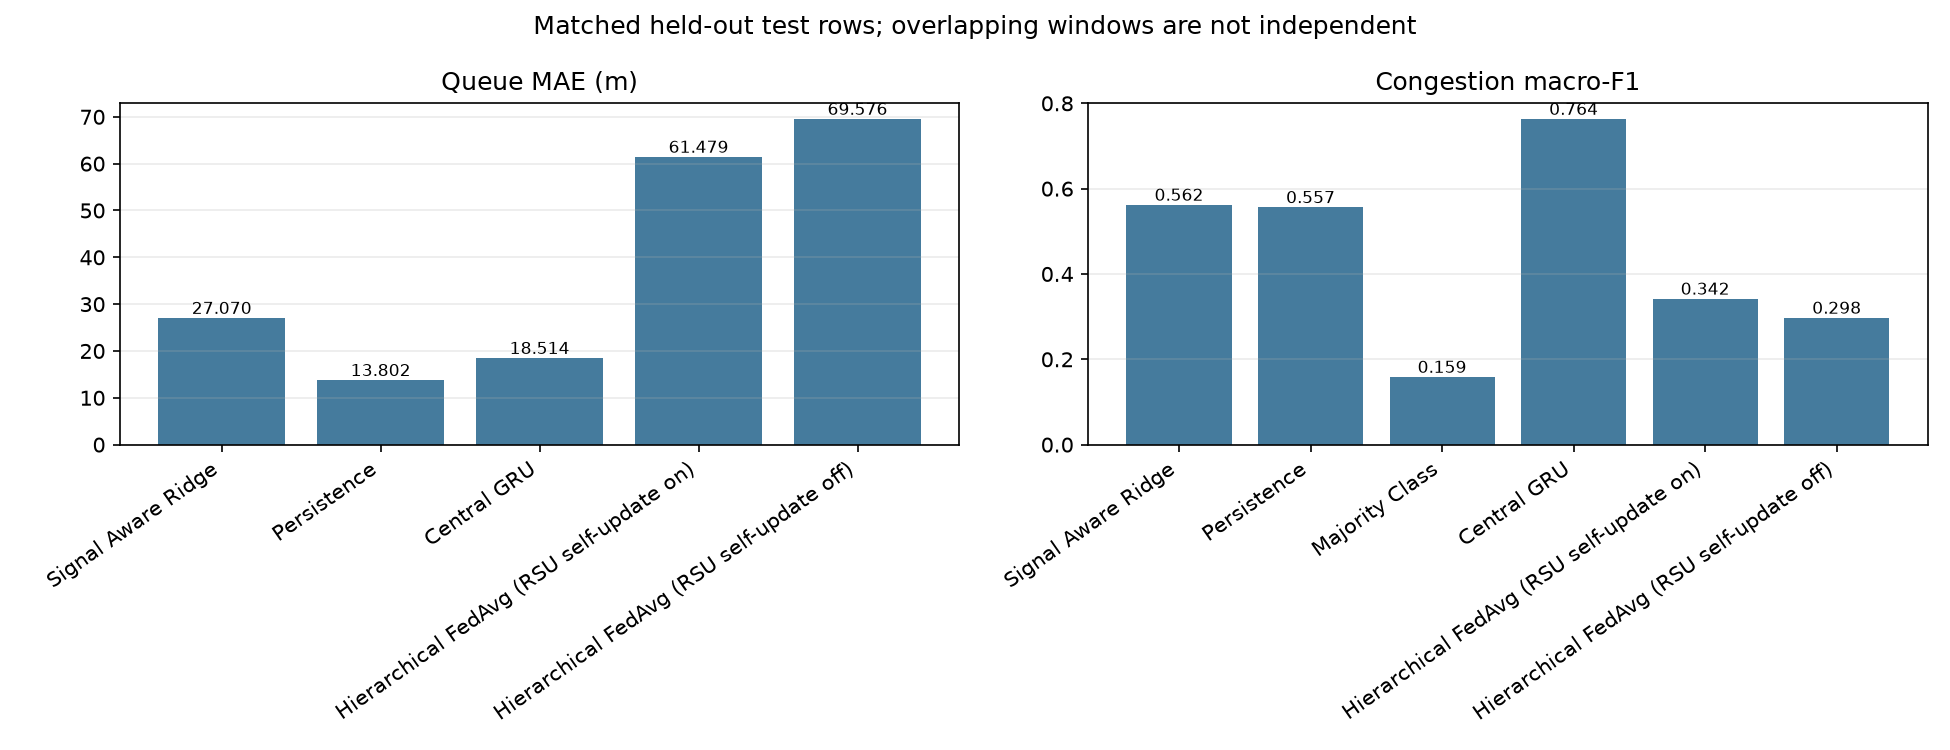
\includegraphics[width=\linewidth]{figs/current_matched_metrics.png}}{\fbox{\parbox{0.8\linewidth}{Matched-metrics figure unavailable in the source folder.}}}
\caption{Comparison of saved regression and classification metrics.}
\label{fig:metrics-current}
\end{figure}

The central model improves over the signal-aware ridge on all four listed metrics in this run. Its macro-F1 of 0.764 is notably higher than the majority baseline's 0.159, but the result should be read alongside the class support and the single-seed, overlapping-window design. The persistence row has only 70 RSU examples; its MAE should not be compared as if it had the same evaluation cohort as the 300-row methods.

\section{Central Model Training}
The central GRU's saved training record shows 50 epochs, a best validation checkpoint at epoch 35, and a run duration of 41.32 seconds (29.31 seconds of recorded training time) on CUDA. The configured minimum epoch count was 50, with a maximum of 150 and patience 15. Since training reached the minimum, early stopping did not end the run before epoch 50. Epoch 35 denotes the selected checkpoint, not the epoch at which training stopped.

\section{Federated Comparison}
The RSU-learning-enabled hierarchical run reports MAE 61.48 m and macro-F1 0.342; disabling RSU local learning reports MAE 69.58 m and macro-F1 0.298. The enabled condition is numerically better on all four metrics in this run, but this is not an isolated causal estimate of RSU learning: it includes four additional learning clients and 300 additional training windows. Both conditions use 100 rounds, five local epochs, and the same 100 configured vehicle clients, with the same held-out evaluation cohort.

Recorded wall durations were 1,056.55 seconds for RSU learning on and 1,002.25 seconds for RSU learning off. These are run-specific durations on the recorded environment; they are not a hardware-independent training-time comparison. The result also shows that the present hierarchical setup does not yet match central training quality. Possible contributors include non-IID client data, the small number of training seeds, client/aggregation dynamics, and the current training schedule. The saved experiment does not establish which factor dominates.

\section{Class-Level Errors}
Figure~\ref{fig:confusion-current} shows the current raw-count confusion matrices. The held-out support is imbalanced, with fewer moderate examples. Central GRU correct predictions are 138 free, 29 moderate, and 75 heavy. For hierarchical learning with RSU learning on, the diagonal counts are 63, 5 and 54; with RSU learning off, they are 41, 4 and 63. These raw counts make the small moderate-class diagonal appear faint in a shared color scale; percentages would answer a different question (per-class recall) and are not the values shown in this report.

\begin{table}[ht]
\centering
\caption{Class-level recall and precision derived from the saved confusion counts.}
\label{tab:class-metrics}
\small
\begin{tabular}{llrrr}
\toprule
Model & Measure & Free & Moderate & Heavy\\
\midrule
Central GRU & Recall & 0.914 & 0.527 & 0.798\\
 & Precision & 0.802 & 0.744 & 0.843\\
HFL, RSU learning on & Recall & 0.417 & 0.091 & 0.574\\
 & Precision & 0.594 & 0.263 & 0.309\\
HFL, RSU learning off & Recall & 0.272 & 0.073 & 0.670\\
 & Precision & 0.577 & 0.267 & 0.294\\
\bottomrule
\end{tabular}
\end{table}

The per-class results clarify the aggregate scores. The central GRU identifies free and heavy examples relatively well but has lower moderate recall (0.527). Both federated models have particularly low moderate recall in this held-out split. The RSU-learning-off model has higher heavy recall than free or moderate recall, consistent with its tendency to predict heavy more often. These values are calculated from the 300-row confusion matrices and are specific to the saved test set; they are not population estimates.

The user-facing raw-count view is retained to match the current report artifacts. A row-normalized visualization would put each actual class on a 0--100\% scale and emphasize recall, but would no longer show sample counts. Both views can be useful; this report's table provides per-class recall alongside counts to keep sample size visible.

\begin{figure}[ht]
\centering
\IfFileExists{figs/current_confusion_matrices.png}{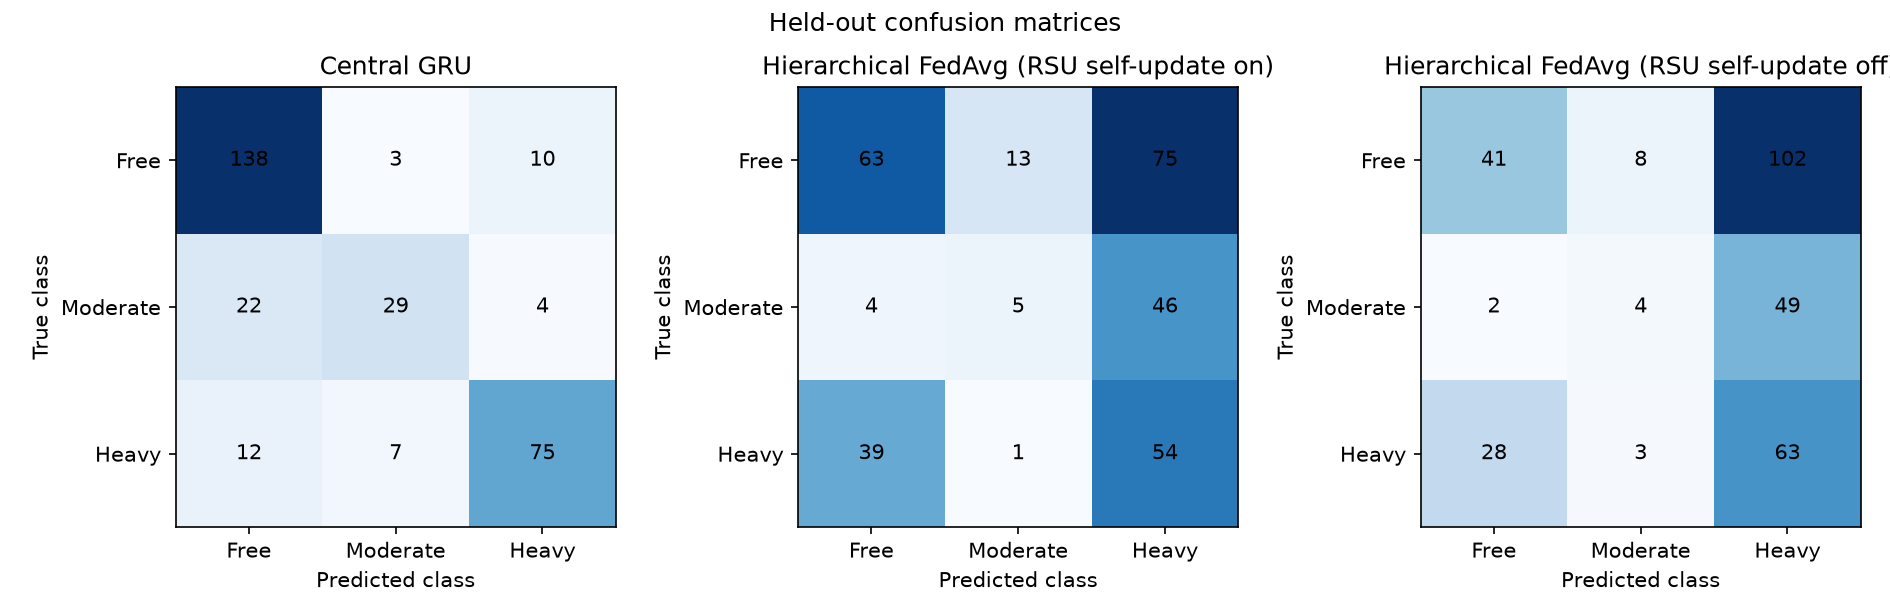
\includegraphics[width=\linewidth]{figs/current_confusion_matrices.png}}{\fbox{\parbox{0.8\linewidth}{Current confusion-matrix figure unavailable in the source folder.}}}
\caption{Raw-count confusion matrices for the central and hierarchical models.}
\label{fig:confusion-current}
\end{figure}

\section{Discussion and Limitations}
The results support the central GRU as a useful predictive baseline for the present compact simulation, not as a validated traffic deployment. The hierarchical experiments prove that the configured training path produces evaluated models, but their scores are lower than the central run. More balanced and repeated experiments are needed before attributing this gap to a specific federation design.

The experiment covers four synthetic demand scenarios at one intersection and one held-out seed per scenario. It has 300 test windows, one model-training seed, and stride-one overlapping examples. The 100-client experiment is based on configured software clients; it does not model 100 physical devices or communication faults. No real sensor data, external intersection, attack, trust intervention, or signal-control outcome is evaluated. The dataset's class distribution and observed errors should therefore be described as properties of this simulation and split.

Natural client heterogeneity is expected because vehicles and RSUs receive different bounded observations, and clients occupy different approaches and see different demand histories. Vehicles on the same approach are not automatically independent: they share the same simulated traffic stream and intersection signal. Accordingly, the effective diversity of 100 vehicle IDs is not equivalent to 100 unrelated data sources. A useful follow-up is to report per-client sample counts and label distributions, quantify between-client divergence, and compare vehicle-only, RSU-only and mixed-client training under equalized example counts.

\section{Interpretation of Queue Forecast Errors}
Queue MAE is the average absolute distance between the predicted and reference queue lengths; an MAE of 18.51 m for the central model means an average absolute error of that size on this particular test cohort. RMSE penalizes larger misses more strongly, so the central model's 28.28 m RMSE being above its MAE indicates a contribution from larger errors. These measures describe continuous queue forecasts and do not tell whether a class boundary was crossed. Conversely, macro-F1 and balanced accuracy summarize classification quality but do not indicate how many metres a queue estimate missed. Reporting both task types is therefore necessary for this multi-output model.

Classification errors can arise from small queue estimation differences near a class threshold. The class label is derived from a queue-length ratio, with boundaries at 0.10 and 0.35; a modest continuous error can change a class when the target lies close to one of those boundaries. A future analysis should report regression error by true class and distance-to-boundary, in addition to the confusion matrix. That would distinguish broad forecasting error from threshold sensitivity. The present saved report does not contain that breakdown, so this explanation is a methodological interpretation rather than a measured causal account of the observed misses.

The central model's improvement over the signal-aware ridge suggests that the sequence model learned useful temporal patterns in this simulation. It does not show that recurrence is inherently superior to other architectures: no equal-budget temporal convolution or transformer comparison is included. The GRU is the implemented model and serves as the first learned reference. Likewise, the hierarchical model's weaker scores should not be read as evidence that federation itself necessarily harms prediction. The present settings differ in data allocation and contain only one training seed. A controlled follow-up should first match the training windows and local optimization budget, then vary only the aggregation or participation rule.

For an operational interpretation, the most important limitation is the observation contract. A vehicle does not directly see the entire approach queue, and its assigned RSU does not change when it exits the junction. The model predicts an approach-level future label from the local view represented in the dataset. This supports studying distributed prediction under restricted views, but it does not yet test seamless infrastructure handoff or real sensor coverage. Those system behaviours must be implemented and validated before relating these offline metrics to continuous roadside service.

The results are suitable as a reproducible starting point for the next experiment: repeat training over multiple seeds, include more held-out runs, and compare central and federated methods under matched example budgets. Additional ablations should separately vary RSU learning, client participation, local epochs and aggregation so that each effect can be interpreted.

%===================================================Chapter5=================================================================
\chapter{CONCLUSION AND FUTURE WORK}\label{ch:conclusion}

\section{Conclusion}
This report documents the implemented TRAF-MA baseline: a left-hand, single-intersection SUMO simulation with four persistent RSU software agents, configurable vehicle agents, bounded observations, a common sequence predictor and hierarchical FedAvg training. The current compact dataset represents four demand scenarios. The evaluated model predicts its own approach queue length and congestion class 30 seconds ahead from ten observations.

This baseline is an implementation stage toward the continuing project problem and objectives stated in Chapters~\ref{ch:intro} and~\ref{ch:survey}. In particular, the current results do not replace the planned work on trust, trust-aware aggregation and consensus, attack robustness, trust recovery or dashboard-based end-to-end evaluation.

On the saved 100-vehicle held-out evaluation, the central GRU achieved MAE 18.51 m, RMSE 28.28 m, macro-F1 0.764 and balanced accuracy 0.746 over 300 overlapping examples. The hierarchical runs with RSU learning on and off achieved lower scores. The enabled run was better numerically than the disabled run, but it also included four additional learning clients and more training examples. These findings are descriptive for one training seed and the current simulation; they do not establish generalisation to real roads or physical sensors.

\section{Limitations}
The implementation uses synthetic SUMO observations at one intersection, fixed-time signal control, and one held-out seed per scenario. The test windows overlap and the moderate class has fewer examples. The current simulation lifecycle does not hand off a vehicle's parent RSU after it crosses the junction. RSUs are software agents and no camera or radar hardware is represented. Trust scoring, attacks, quarantine, physical signal control and a live operational dashboard are outside the completed work reported here.

\section{Future Work}
The next phase should first improve evaluation reliability: train multiple seeds, expand held-out runs, report per-class precision and recall, and use run-level uncertainty intervals. Central and hierarchical comparisons should use matched data budgets, with separate ablations for vehicle updates, RSU updates, local epochs and client participation. Alternative sequence architectures such as a temporal convolutional network can then be compared under the same features, splits and compute budget.

Simulation extensions should evaluate route-aware transfer between RSUs at the junction, clearer inbound/outbound sensing rules, and larger networks with varied signal timing. SUMO detectors such as E2 can be represented as an explicit simulated sensor interface if detector-level observations are added; this would still not imply physical hardware. Finally, trust and security mechanisms should be implemented as a separate milestone with controlled attacks, benign non-IID clients, transparent evidence, quarantine/recovery tests and matched clean baselines. Real-world claims require external data and validation beyond the current simulator.


% References, Appendix and Timeline (hand-written thebibliography lives in ref.tex;
% the old \bibliography{ref.bib} call pointed at unused template entries, so it was removed)
\cleardoublepage
\renewcommand{\bibname}{KEY REFERENCES}
\begin{thebibliography}{13}
\small
\bibitem{chellapandi2023}
V.~P. Chellapandi, L.~Yuan, C.~G. Brinton, S.~H. Zak, and Z.~Wang,
Federated learning for connected and automated vehicles: A survey of existing approaches and challenges,
\emph{IEEE Transactions on Intelligent Vehicles}, vol.~9, no.~1, pp.~119--137, 2024, doi:10.1109/TIV.2023.3332675.

\bibitem{zhang2024}
R.~Zhang, H.~Wang, B.~Li, X.~Cheng, and L.~Yang,
A survey on federated learning in intelligent transportation systems,
arXiv:2403.07444, 2024.

\bibitem{babar2026}
M.~Babar, B.~Qureshi, W.~Boulila, and A.~Koubaa,
Federated learning for intelligent transportation systems: Emerging trends, challenges and future directions,
\emph{Computer Science Review}, 2026, doi:10.1016/j.cosrev.2026.100952.

\bibitem{subbulakshmi2025}
V.~Subbulakshmi, S.~Chaudhari, and S.~Pathan,
Federated learning-based travel time prediction for adaptive congestion control using 5G-assisted roundabout traffic networks,
\emph{IEEE Access}, vol.~13, pp.~156389--156406, 2025, doi:10.1109/ACCESS.2025.3605987.

\bibitem{shit2025}
R.~C. Shit and S.~Subudhi,
Privacy-preserving federated learning for fair and efficient urban traffic optimization,
arXiv:2511.06363, 2025.

\bibitem{amari2023}
H.~Amari, Z.~Abou El Houda, L.~Khoukhi, and L.~H. Belguith,
Trust management in vehicular ad-hoc networks: Extensive survey,
\emph{IEEE Access}, vol.~11, pp.~47659--47680, 2023, doi:10.1109/ACCESS.2023.3268991.

\bibitem{tian2025}
R.~Tian, J.~Mei, and G.~Ma,
Privacy-preserving resilient consensus for delayed multi-agent systems: A scheme via trusted nodes,
\emph{Systems \& Control Letters}, vol.~203, art.~106167, 2025, doi:10.1016/j.sysconle.2025.106167.

\bibitem{zafar2025}
U.~Zafar, A.~M.~H. Teixeira, and S.~Toor,
Byzantine-robust federated learning using generative adversarial networks,
arXiv:2503.20884, 2025.

\bibitem{mcmahan2017}
B.~McMahan, E.~Moore, D.~Ramage, S.~Hampson, and B.~A. y Arcas,
Communication-efficient learning of deep networks from decentralized data,
in \emph{Proceedings of AISTATS}, 2017, pp.~1273--1282.

\bibitem{lopez2018}
P.~A. Lopez et al., Microscopic traffic simulation using SUMO,
in \emph{Proceedings of the IEEE International Conference on Intelligent Transportation Systems}, 2018, pp.~2575--2582.

\bibitem{wegener2008}
A.~Wegener et al., TraCI: An interface for coupling road traffic and network simulators,
in \emph{Proceedings of the 11th Communications and Networking Simulation Symposium}, 2008.

\bibitem{cho2014}
K.~Cho et al., Learning phrase representations using RNN encoder-decoder for statistical machine translation,
in \emph{Proceedings of EMNLP}, 2014, pp.~1724--1734.
\end{thebibliography}

\chapter*{PROJECT TIMELINE}
\addcontentsline{toc}{chapter}{PROJECT TIMELINE}
\begin{table}[ht]
\centering
\caption{Project timeline and implementation status at report preparation.}
\begin{tabular}{p{0.18\linewidth}p{0.58\linewidth}p{0.16\linewidth}}
\toprule
Period & Work package & Status\\
\midrule
Phase 1 & SUMO intersection, bounded agents, observation and message contracts & Implemented\\
Phase 2A & Dataset generation, local targets, central GRU and baseline evaluation & Implemented\\
Phase 2B & Vehicle-to-RSU-to-coordinator hierarchical FedAvg and RSU ablation & Implemented; results limited\\
Next phase & Multi-seed evaluation, route-aware RSU handoff and matched-budget ablations & Planned\\
Next phase & Trust/security experiments, attacks, quarantine/recovery and dashboard & Planned\\
\bottomrule
\end{tabular}
\end{table}

\newpage


\end{document}
